\documentclass[12pt]{article} % Default font size is 12pt, it can be changed here
\usepackage[portuguese]{babel}
\usepackage[utf8]{inputenc}
\usepackage[T1]{fontenc}
\usepackage{color}
\usepackage{indentfirst}

\usepackage{geometry} % Required to change the page size to A4
\geometry{a4paper} % Set the page size to be A4 as opposed to the default US Letter

\usepackage{graphicx} % Required for including pictures

% (1) choose a font that is available as T1
% for example:
\usepackage{lmodern}

% (2) specify encoding
\usepackage[T1]{fontenc}

% (3) load symbol definitions
\usepackage{textcomp}
\usepackage{float} % Allows putting an [H] in \begin{figure} to specify the exact location of the figure
\usepackage{wrapfig} % Allows in-line images such as the example fish picture

\usepackage{listings} % Para codigo cenas
\usepackage{array}
\usepackage{url}
\linespread{1.2} % Line spacing

\graphicspath{{./Pictures/}} % Specifies the directory where pictures are stored
\usepackage{fancyhdr}
\pagestyle{fancy}

\begin{document}
\lhead{Sistemas Distribuídos}
\rhead{Projecto 1}
%--------------------------------------------------------------------------
%	TITLE PAGE
%-------------------------------------------------------------------------

\begin{titlepage}

\newcommand{\HRule}{\rule{\linewidth}{0.5mm}} % Defines a new command for the horizontal lines, change thickness here

\center % Center everything on the page

\textsc{\LARGE Universidade de Coimbra}\\[1.5cm] % Name of your university/college
\textsc{\Large Licenciatura Engenharia Informática\\2014-2015}\\[0.5cm] % Major heading such as course name

\HRule \\[0.4cm]
{\huge \bfseries Sistemas Distribuídos - Projeto 1}\\[0.4cm] % Title of your document
\HRule \\[1.5cm]

\begin{minipage}{0.8\textwidth}

\begin{flushleft} \large
\emph{Autores:}\\
Bruno \textsc{Martins} - Nº2007183389
\end{flushleft}

\end{minipage}

\begin{minipage}{0.4\textwidth}
\begin{flushright} \large
\end{flushright}
\end{minipage}\\[4cm]

{\large \today}\\[3cm] % Date, change the \today to a set date if you want to be precise
\vfill % Fill the rest of the page with whitespace

\end{titlepage}

%--------------------------------------------------------------------------
%	TABLE OF CONTENTS
%--------------------------------------------------------------------------
\tableofcontents % Include a table of contents



\newpage % Begins the essay on a new page instead of on the same page as the table of contents 

%--------------------------------------------------------------------------
%	INTRODUCTION
%--------------------------------------------------------------------------

\section{Introdução} % Major section
\label{sec:intro}
O presente relatório destina-se a apresentar a descrição do projecto 1 da cadeira de Sistemas Distribuídos intitulado \emph{Meeto – Collaboration and Social Networking}.\\

Reuniões são necessárias quando diversas pessoas trabalham em conjunto. Alunos reunem-se para coordenar o seu esforço nos trabalhos práticos; trabalhadores reunem-se para discutir o estado dos projectos e gestores reunem-se para tomar decisões chave relacionadas com as suas organizações e por aí fora. É necessário um sistema que impeça as pessoas de gastarem tempo desnecessário em reuniões. Afinal de contas, tempo é o nosso recurso mais valioso.

Este projecto consiste então numa implementação de um sistema de gestão de reuniões, onde os utilizadores podem criar reuniões, convidar participantes, ter uma sala de chat para cada tópico da reunião e no final adicionar decisões chave a cada reunião. É também possível relacionar pessoas a certas tarefas - uma vez que uma reunião sem atribuição de tarefas concretas aos seus elementos de pouco serve.

\begin{figure}[!ht]
  	\centering
  	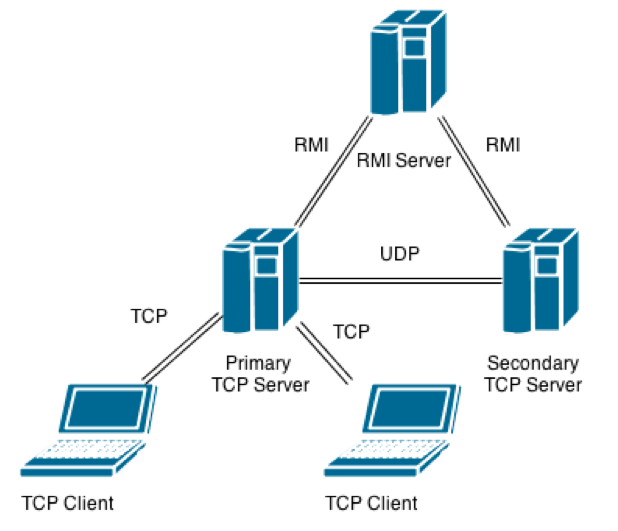
\includegraphics[scale=0.5]{figure1.png}
  	\caption{Visão Global da Arquitectura}
	%\vspace{2cm}
	\label{figure1}
\end{figure}


%--------------------------------------------------------------------------
%	INTERNAL ARCHITECTURE
%--------------------------------------------------------------------------
\section{Internal architecture}
\label{sub:internal}

Esta aplicação encontra-se subdividida numa série de classes, cada uma responsável por integrar esta aplicação num todo coerente, onde se destacam:

\begin{description}
	\item[RMIServer:] \hfill \\
	Dentro da classe \textbf{RMIServer} encontram-se os métodos essenciais da aplicação: registo, login, createMeeting, listAllMeetings, acceptMeeting, meetingOverview, addAgendaItem etc. É aqui que é criado o registry e onde é instanciado o objecto para ligação à base de dados MySQL. Dentro do RMIServer são também chamados vários métodos do TCPServer (callback), entre eles o \textbf{msgToMany} que trata de enviar uma mensagem a vários destinatários e o \textbf{msgsToOne} que envia diversas mensagens para o mesmo utilizador. Relativamente a threads, o RMI faz uma gestão interna automática das mesmas.

	\item[RmiInterface:] \hfill \\
	O RmiInterface, tal como o próprio nome indica, é a interface dos métodos existentes dentro da RMIServer.
	\item[MySQL:] \hfill \\
	Classe onde se encontram os métodos para ligação à base de dados MySQL e para correcta execução dos diferentes tipos de queries.
	\item[TCPServer:] \hfill \\
	Interface dos métodos existentes dentro do TCPServerImpl
	\item[TCPServerImpl:] \hfill \\
	Implementa os métodos da interface e é aqui onde os clientes se ligam (abrindo dois sockets e mais duas threads para cada um). Possui 2 threads internas (UDP Sender e UDP Receiver) e guarda a relação entre users e threads numa HashTable. Correndo o ficheiro duas vezes simula a arquitectura desejada (tcp server primário e tcp server de backup).	
	\item[TCPClient:] \hfill \\
	Este cliente estabelece a ligação com o servidor através de dois Sockets TCP (uma para pedidos request-reply e outro para eventos em "tempo real") promovendo não só a construção dos menus (menu de login, inicial, etc.) como também a arquitetura da aplicação melhorando, deste modo, a comunicação com o servidor. É responsável por providenciar informação e dados através da criação de mensagens, como também requisita serviços à aplicação, como por exemplo listar meetings existentes, ou comprar aceitar convites.
	Possui internamente uma thread para ler dados que surjam sem ser necessário uma interacção do utilizador com o sistema.

\end{description}

Estas classes são responsáveis por estabelecer grande parte da interoperabilidade desta aplicação embora sejam necessárias as restantes que suportam a estrutura por detrás deste sistema.\\ 


Relativamente ao armazenamento de dados na Base de Dados, foram criadas as tabelas:

\begin{figure}[!ht]
  	\centering
  	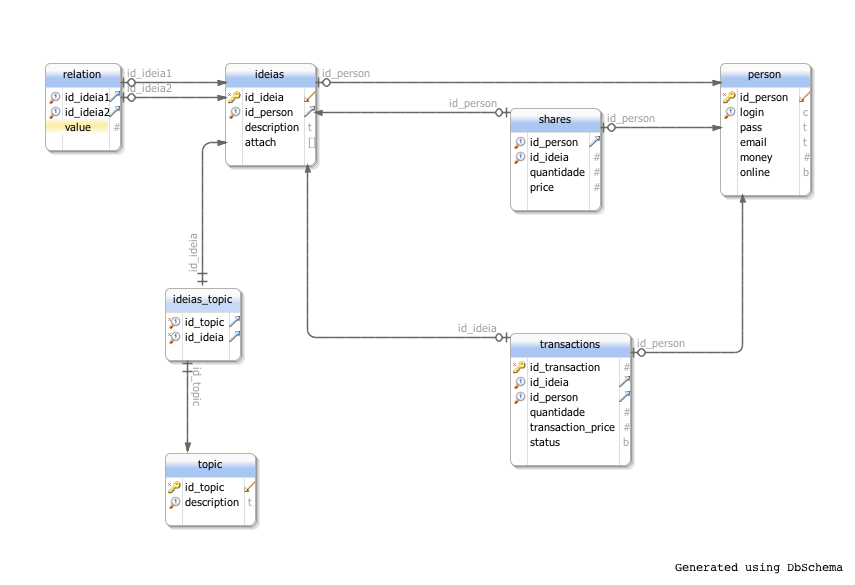
\includegraphics[scale=0.5]{ERdiagram.png}
  	\caption{Diagrama Entidade Relacionamento}
	%\vspace{2cm}
	\label{figure3}
\end{figure}

\-
\pagebreak


%--------------------------------------------------------------------------
%	DATA MODEL
%--------------------------------------------------------------------------
\section{Data model} % 
\label{sec:data}
O seguinte diagrama representa o nosso esquema de Data Model.

\begin{figure}[!ht]
  	\centering
  	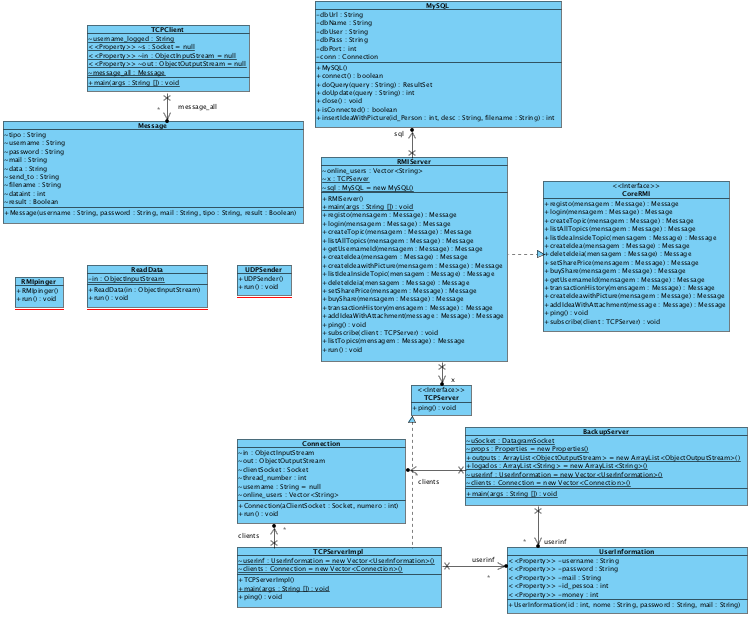
\includegraphics[scale=0.2]{ClassDiagram.png}
  	\caption{Data Diagram}
	%\vspace{2cm}
	\label{figure4}
\end{figure}

Todo o tipo de requests, acções e triggers no projecto são acionados a partir do instanciamento de variáveis da classe "Message" - são estes os objectos que circulam na rede. Possui diversos construtores que se podem usar consoante a acção a tomar. O tratamento correcto das mensagens é feito através da inspecção do parâmetro "type".





%--------------------------------------------------------------------------
%	Protocol Specification (TCP, UDP, RMI)
%--------------------------------------------------------------------------
\section{Protocol Specification (TCP, UDP, RMI)} % 
\label{sec:protocal_specs}

\subsection{TCP}

Ao serem iniciados, os servers TCP criam dois ServerSockets e ficam à espera de ligações de clientes. Assim que estes se ligam, são criadas duas threads que irão tratar dos pedidos dos e para os clientes: A thread Connection, que irá servir principalmente para tipo de pedidos request reply (listagem de meetings, por exemplo), e a thread Events, que irá servir para enviar informação em "real-time" (thread para enviar mensagens que não são necessáriamente solicitadas pelos clientes). Estas threads façam o lookup do Registry do RMI e chamam os seus métodos consoante necessário.

Aqui também se encontra uma Hastable que relaciona os membros online com as suas threads de Events - para o servidor RMI fazer callback do método que envia as mensagens (e.g chat) aos diversos utilizadores e o TCP Server saber que thread corresponde a cada user.

É aqui também que é realizada a verificação do primary server e  do backup server através do método "validadeIfMaster" (que lança uma custom exception ~\textbf{NotMasterException} caso não seja.


\subsection{UDP}

Correndo o TCP server em máquinas diferentes (ou duas vezes na mesma máquina) consegue-se simular o comportamento de um server primário e de um server secundário. Estes comunicam entre sim através de duas threads: UDP Sender e UDP Receiver. Quando o UDP receiver deixa de receber heartbeats, espera alguns segundos até começar a receber clientes.


\subsection{RMI}
O Java RMI(Remote Method Invocation) usa uma metodologia diferente da do TCP. Ao contrário deste, não é estabelecido directamente um canal de comunicação como no TCP em que o servidor está a escuta num determinado porto e para cada cliente cria um socket.
Especificamente, neste projecto o RMI é o nosso main-server, sendo este responsável pelos métodos existentes em toda a sua envolvente. Torna-se assim também o nosso \textbf{single point of failure}.
Assim que é iniciado é criado o registry para os diversos recursos do programa poderem chamar os seus métodos. 


%--------------------------------------------------------------------------
%	Exception Handling
%--------------------------------------------------------------------------
\section{Exception Handling}
\label{sec:except}

No que toca a tratamentos de excepção, foi assegurado que um Cliente reconecta ao mesmo servidor em caso de falha temporária do TCPServer (através de um tempo de espera), sendo a falha transparente para o usuário final.
Através do uso de base de dados, o TCPClient não perde a ideia que está sendo escrita.
O TCPServer reconecta em caso de perda de conectividade com o RMIServer e 
a falha transitória da RMIServer é transparente para o usuário final.
Também houve o cuidado da verificação e foi assegurado que não existem operações duplicadas. duplicadas.

\subsection{A nível de Base de Dados}
O tratamento de erros do nosso MySQL é baseado em condições, que por sua vez, são nomeadas e preparadas para serem executadas mediante ao atendimento de tais condições. 
Além de tratarmos a violação de chaves primárias, foi tido em conta que os ids não assumam valores nulos (NULL), assim como houve um cuidado para que estes fossem auto-incrementáveis. Ao definir corretamente todas as relações e entidades fracas, foi possível haver um relacionamento directo entre entidades de diferentes campos. Foi dado \textbf{cascade} em operações de \emph{update} e \emph{delete}, para que os dados entre tabelas se mantenham coerentes. 


\subsection{TCP}
De modo a tornar esta aplicação ao mesmo tempo transparente a erros e eficiente no seu tratamento procurámos controlar as exceções provenientes dos mecanismos de conexão (Sockets, RMI registry, etc.). Estes problemas advêm de falhas de ligação entre o servidor e o cliente, de uma ruptura do socket TCP, etc.
Implementámos diversas rotinas para gerir estas exceções (try/catch (IO Exception, Remote Exception)) em ambas as ‘extremidades’ da aplicação. As threads responsáveis por estas funções (ConnectBackupServer, UDP) permitem não só isolar o tratamento destas situações, podendo o cliente continuar a usar a aplicação (com algumas restrições), como também restabelecer as ligações entre as entidades executantes ou, em caso de insucesso, ativar um backup. 
Quando o servidor deixa de funcionar correctamente, vai ser detectada uma falha. O cliente irá então tentar voltar a conectar-se, sendo a função udpsender() a responsável pelas tentativas.
Na tentativa do Cliente se conectar ao Servidor, este efetua uma espera de um intervalos de 3 segundos entre cada tentativa de conexão. Entretanto, caso o cliente tente realizar algum pedido, a thread destinada à escrita de teclado fica bloqueada até este realizar re-connect.

\subsection{RMI}
No RMI foram dados os mesmos tratamentos de exceção utilizados no TCP.


\pagebreak

%--------------------------------------------------------------------------
%	FailOver
%--------------------------------------------------------------------------
\section{FailOver}
\label{sec:failover}
O fail-over pressupõe a existência de dois servidores (primary e backup) que comunicam entre si através de um canal UDP. Só assim é possível controlar o estado (ativo/inativo) de cada uma das entidades e efetuar a troca em caso de necessidade. Para tal, operámos um mecanismo de hearbeats (2s).Se depois de 10 segundos o server em utilização não comunicar, os clientes serão redirecionados para o servidor secundário que assumirá o papel de principal.

\pagebreak
%--------------------------------------------------------------------------
%	Strict Order Implementation
%--------------------------------------------------------------------------
\section{Causal Order Implementation}
\label{sec:causal}

Para implementar a ordem causal no projecto foi utilziada um LinkedBlockingQueue em cada thread de Events. Assim que o server RMI pretende enviar mensagens para N utilizadores, faz callback do método sendMsg do TCP Server. Este limita-se a ver se os destinatários estão na sua Hashtable e faz \textbf{offer} às mensagens para a LinkedBlockingQueue. A thread Events está então responsável por ler o conteúdo da LinkedBlockingQueue e enviar para o seu cliente.

\pagebreak
%--------------------------------------------------------------------------
%	Description of tests (Table with Pass/Fail)
%--------------------------------------------------------------------------
\section{Description of tests (Table with Pass/Fail)} % (fold)
\label{sec:Tests}
Foram feitos diversos testes nas diversas funcionalidades da aplicação, de modo a assegurar a robustez da aplicação garantindo, assim, um sistema seguro e eficiente, procurámos testá-lo minuciosamente.

%%%%%%%%%%%%%%%%%%%%%%%%%%%%%%%%%%%%%%%%%%%%%%%%---------------REGISTER
\subsection{Teste de Registo}
\begin{table}[ht!]
	\begin{tabular}{|c|p{4cm}|p{4cm}|p{3cm}|p{1cm}|}
		\hline
		\multicolumn{5}{|l|}{\textbf{Test Name}: Registar}\\
		\hline
		\multicolumn{5}{|l|}{\textbf{Description}: Registo do cliente na BD da aplicação}\\
		\hline
		\multicolumn{5}{|p{14,5cm}|}{\textbf{Prerequisites}: O cliente tem de entrar na aplicação e escolhe a opção REGISTAR}\\
		\hline
		\multicolumn{5}{|l|}{\textbf{Setup}: O cliente cria uma nova conta}\\
		\hline
		\textbf{Step} & \textbf{Operator Action} & \textbf{Expected Results} & \textbf{Observed Results} & \textbf{Pass / Fail}\\
		\hline
		1 & Escolhe a opção Registar & Sistema abre os campos de registo & São os esperados & PASS\\
		\hline
		2 & Inserir username, password e email & Sistema aceita dados e guarda na BD ou rejeita caso o username escolhido já esteja a ser utilizado & São os esperados & PASS\\
		\hline
	\end{tabular}
\end{table}
\pagebreak


%%%%%%%%%%%%%%%%%%%%%%%%%%%%%%%%%%%%%%%%%%%%%%%%---------------LOGIN
\subsection{Teste de Login}
\begin{table}[ht!]
	\begin{tabular}{|c|p{4cm}|p{4cm}|p{3cm}|p{1cm}|}
		\hline
		\multicolumn{5}{|l|}{\textbf{Test Name}: Login}\\
		\hline
		\multicolumn{5}{|l|}{\textbf{Description}: Identificação do cliente}\\
		\hline
		\multicolumn{5}{|p{14,5cm}|}{\textbf{Prerequisites}: Cliente tem de ter uma conta criada na aplicação}\\
		\hline
		\multicolumn{5}{|l|}{\textbf{Setup}: O cliente insere a sua pass e username para usar a sua conta}\\
		\hline
		\textbf{Step} & \textbf{Operator Action} & \textbf{Expected Results} & \textbf{Observed Results} & \textbf{Pass / Fail}\\
		\hline
		1 & Inserir username, password & Sistema aceita dados se essa conta existir & São os esperados & PASS\\
		\hline
	\end{tabular}
\end{table}
\pagebreak

%%%%%%%%%%%%%%%%%%%%%%%%%%%%%%%%%%%%%%%%%%%%%%%%---------------IDEIA
\subsection{Teste de criação de meeting}
\begin{table}[ht!]
	\begin{tabular}{|c|p{4cm}|p{4cm}|p{3cm}|p{1cm}|}
		\hline
		\multicolumn{5}{|l|}{\textbf{Test Name}: Teste de Submissão de Meeting}\\
		\hline
		\multicolumn{5}{|p{14,5cm}|}{\textbf{Description}: É testada a funcionalidade de introduzir meeting}\\
		\hline
		\multicolumn{5}{|p{14,5cm}|}{\textbf{Prerequisites}: O utilizador tem que já estar registado}\\
		\hline
		\multicolumn{5}{|p{14,5cm}|}{\textbf{Setup}: O servidor irá fazer handle das meetings}\\
		\hline
		\textbf{Step} & \textbf{Operator Action} & \textbf{Expected Results} & \textbf{Observed Results} & \textbf{P / F}\\
		\hline
		1 & logar User & Login efectuado com sucesso! & Nada apontar & PASS\\
		\hline
		2 & User acede ao menu e escolhe a opção 1 & aparece o passo seguinte & antes de escolher a opção, aparece uma listagem de opções & PASS\\
		\hline
		3 & Introduz os detalhes da meeting & wfsgg & nada apontar & PASS\\
		\hline
		4 & Escolhe a opção de sim relativamente ao anexo & Passa ao passo seguinte & é introduzido a path do anexo & PASS\\
		\hline
		5 & --- & Passa À seguinte pergunta relativamente a adicionar a ideia a um tópico & pergunta se deseja introduzir um novo tópico ou usar os existentes & PASS\\
		\hline
		6 & Escolhe a opção de usar tópicos existentes & Lista todos os tópicos existentes & nada apontar & PASS\\
		\hline
		7 & Vai introduzir os tópicos 1 e 2 e por fim clica em 0 para finalizar & Ir pedindo mais tópicos enquanto não se clica na tecla 0 & É introduzida a associação da ideia com o tópico, com sucesso & PASS\\
		\hline
	\end{tabular}
\end{table}
\pagebreak



%%%%%%%%%%%%%%%%%%%%%%%%%%%%%%%%%%%%%%%%%%%%%%%%---------------CONECTAR A BACKUP
\subsection{Teste de Ligação ao Servidor Backup}
\begin{table}[ht!]
	\begin{tabular}{|c|p{4cm}|p{4cm}|p{3cm}|p{1cm}|}
		\hline
		\multicolumn{5}{|l|}{\textbf{Test Name}: Ligação ao Servidor Backup}\\
		\hline
		\multicolumn{5}{|l|}{\textbf{Description}: Teste de Ligação ao Backup}\\
		\hline
		\multicolumn{5}{|p{14,5cm}|}{\textbf{Prerequisites}: Cliente tem de ter uma conta criada na aplicação e devem estar os dois servidores a correr. Será feita uma ligação normal entre cliente TCP e Servidor TCP. De seguida será quebrada a ligação do servidor principal TCP, esperando assim que o cliente se reconecte ao servidor backup}\\
		\hline
		\multicolumn{5}{|l|}{\textbf{Setup}: Acesso normal À sua conta}\\
		\hline
		\textbf{Step} & \textbf{Operator Action} & \textbf{Expected Results} & \textbf{Observed Results} & \textbf{Pass / Fail}\\
		\hline
		1 & Inserir username, password & Sistema aceita dados se a conta existir & São os esperados & PASS\\
		\hline
		2 & O servidor principal é desligado & Existe um período de espera da parte do cliente até este se ligar ao servidor backup, podendo ter existido um curto downtime da parte do principal & O servidor principal não vem up dentro o tempo de espera & PASS\\
		\hline
		3 & ---- & Ligação feita ao servidor backup & São os esperados & PASS\\
		\hline
	\end{tabular}
\end{table}




\newpage
%--------------------------------------------------------------------------
%	Manual de Instalação
%--------------------------------------------------------------------------
\section{Manual de Instalação}
\label{sec:install}
Para correr a aplicação irá necessitar dos seguintes requisitos:
\begin{itemize}
	\item Java 8
	\item Servidor com MySQL com a respectiva base de dados (o script de criação da base de dados encontra-se na pasta support, ficheiro \emph{meetosqlscript.sql}
\end{itemize}

Após reunidos todos os requisitos necessários, é necessário que o MySQL esteja a correr dentro da própria (localhost), ou no caso que esteja se encontre noutra máquina, que seja definido o respectivo IP e porta.
Como foi mencionado anteriormente, deve-se correr o script \emph{meetossqlcript.sql} que contem todas as tabelas criadas bem como alguns dados.
Por fim, deve-se executar-se por esta ordem a execução de servidores da máquina:

\begin{itemize}
	\item 1 - RMIServer.java
 	\item 2 - TCPServer.java (duas vezes para simular o comportamento de servidor primário e secundário)
	\item 3 - TCPClient.java (quantas vezes necessário para criar vários clientes)
\end{itemize}

Relativamente ao IP de máquina onde os servidores e o cliente estão a correr, existe um ficheiro intitulado \emph{property} (support/property) onde se pode alterar os endereços e as portas onde estes vão estar a correr.

\begin{verbatim}
tcpip1=127.0.0.1
tcpip2=127.0.0.1
tcpServerPort=7000
tcpServerPortAux=7001
tcpBackupServerPort=7002
tcpBackupserverPortAux=7003
udpPort=5432
rmiServerip=127.0.0.1
rmiServerPort1=1099
rmiServerPort2=6001


\end{verbatim}


E... pronto! É só escolher as operações pretendidas!



\end{document}